%!TEX program = xelatex
% ==============================================================================
% AA CONFIGURAZIONE DI BASE ED ENGINE
% ==============================================================================
% BB CLASSE DEL DOCUMENTO
\documentclass[11pt, a4paper]{article}

% ==============================================================================
% AA LINGUA, FONT E TIPOGRAFIA
% ==============================================================================
% BB GESTIONE FONT XELATEX
\usepackage{fontspec}
\setmainfont{Latin Modern Roman}

% BB LOCALIZZAZIONE LINGUISTICA
\usepackage[italian]{babel}

% BB TIPOGRAFIA E MICRO-ESTENSIONI
\usepackage[protrusion=true]{microtype}
\raggedbottom

% ==============================================================================
% AA LAYOUT DI PAGINA E SPAZIATURA PARAGRAFI
% ==============================================================================
% BB GEOMETRIA DEI MARGINI
\usepackage[left=2.4cm, right=1.6cm, top=2cm, bottom=2cm]{geometry}

% BB CONTROLLO SPAZIATURA TRA PARAGRAFI
\usepackage[skip=3pt plus 1pt minus 1pt]{parskip}

% ==============================================================================
% AA MOTORE DEI COLORI E MACRO LOCALI
% ==============================================================================
% BB CARICAMENTO CORE XCOLOR IN SPAZIO GRAY PURO
\usepackage[gray]{xcolor}

% ==============================================================================
% AA MATEMATICA E SIMBOLI SCIENTIFICI
% ==============================================================================
% BB PACCHETTI MATEMATICI UNICODE
\usepackage{mathtools}
\usepackage[warnings-off={mathtools-overbracket,mathtools-colon}]{unicode-math}
\setmathfont{Latin Modern Math}

% BB METRICHE MATRICI E FORMULE DISPLAY
\setlength{\arraycolsep}{10pt}
\setlength{\abovedisplayskip}{3pt plus 1pt minus 1pt}
\setlength{\belowdisplayskip}{3pt plus 1pt minus 1pt}
\setlength{\abovedisplayshortskip}{0pt plus 1pt}
\setlength{\belowdisplayshortskip}{2pt plus 1pt minus 1pt}
\allowdisplaybreaks

% ==============================================================================
% AA GRAFICA ED ELEMENTI FLOTTANTI
% ==============================================================================
% BB MOTORE DI INCLUSIONE GRAFICA E GESTIONE RIGIDA
\usepackage{graphicx}
\graphicspath{{./E3_6_1_Images/}}
\usepackage{float}

% ==============================================================================
% AA TITOLI E STRUTTURA DEL DOCUMENTO (MONOCROMATICI NERI)
% ==============================================================================
% BB PACCHETTO TITLESEC
\usepackage{titlesec}

% BB FORMATTAZIONE TIPOGRAFICA (TITOLI NERI)
\titleformat{\section}{\normalfont\Large\bfseries}{\thesection}{1em}{}
\titleformat{name=\section,numberless}{\normalfont\Large\bfseries}{}{0pt}{}
\titleformat{\subsection}{\normalfont\large\bfseries}{\thesubsection}{1em}{}
\titleformat{name=\subsection,numberless}{\normalfont\large\bfseries}{}{0pt}{}
\titleformat{\subsubsection}{\normalfont\normalsize\bfseries}{\thesubsubsection}{1em}{}
\titleformat{name=\subsubsection,numberless}{\normalfont\normalsize\bfseries}{}{0pt}{}

% BB SPAZIATURA VERTICALE DEI TITOLI
\titlespacing*{\section}{0pt}{1.2ex plus 0.4ex minus 0.2ex}{0.6ex plus 0.2ex}
\titlespacing*{\subsection}{0pt}{1ex plus 0.3ex minus 0.2ex}{0.5ex plus 0.2ex}
\titlespacing*{\subsubsection}{0pt}{0.8ex plus 0.2ex minus 0.1ex}{0.4ex plus 0.1ex}

% ==============================================================================
% AA INTEGRAZIONE AMBIENTE MATLAB
% ==============================================================================
% BB CARICAMENTO PACCHETTO MATLAB
\usepackage{matlab}

% BB ATTIVAZIONE SEGNALIBRI E INDICE MATLAB
\matlabmultipletitles
\matlabhastoc

% ==============================================================================
% AA IPERTESTO, SEGNALIBRI ED ELENCHI
% ==============================================================================
% BB CONFIGURAZIONE HYPERREF E METADATI PDF
\hypersetup{
    hidelinks,
    pdfauthor={Francesco Lo Verde},
    pdftitle={Cinematica diretta manipolatore Stanford}
}

% BB SEGNALIBRI AVANZATI
\usepackage{bookmark}

% BB FORMATTAZIONE ELENCHI PUNTATI E NUMERATI
\usepackage{enumitem}
\setlist{itemsep=3.5pt plus 1pt minus 1pt, topsep=4pt plus 1pt minus 1pt, partopsep=0pt, parsep=1pt}

\begin{document}

\matlabtitle{Cinematica diretta manipolatore di Stanford}

\begin{par}
\begin{flushleft}
L'obiettivo della cinematica diretta è determinare la posizione e l'orientamento dell'organo terminale (end-effector) a partire dai valori delle variabili di giunto. Si utilizza la convenzione di Denavit-Hartenberg (DH) per modellare la geometria del robot. La convenzione di Denavit-Hartenberg è un metodo standard per assegnare sistemi di riferimento ai bracci di un robot. Per ogni braccio, si definiscono quattro parametri che descrivono la trasformazione geometrica rispetto al braccio precedente.
\end{flushleft}
\end{par}

\begin{par}
\begin{flushleft}
Si inizia definendo le variabili simboliche necessarie per i parametri DH. Questo permette di eseguire i calcoli in forma generale, senza dover specificare subito valori numerici. Successivamente, si assemblano questi parametri in una tabella dove ogni riga corrisponde a un giunto del robot e le colonne rappresentano i parametri $\left(\begin{array}{c}
\theta ,d,\alpha ,a
\end{array}\right)$.
\end{flushleft}
\end{par}

\begin{matlabcode}
clc;
clear;
close all;

% Definizione variabili simboliche
syms q1 q2 q3 q4 q5 q6 d2 d6 real;

% Tabella parametri Denavit-Hartenberg (DH)
DH_table = [q1, 0, -pi/2, 0;    % Giunto 1 (0 -> 1)
            q2, d2, pi/2, 0;    % Giunto 2 (1 -> 2)
            0, q3, 0, 0;        % Giunto 3 (2 -> 3)
            q4, 0, -pi/2, 0;    % Giunto 4 (3 -> 4)
            q5, 0, pi/2, 0;     % Giunto 5 (4 -> 5)
            q6, d6, 0, 0];      % Giunto 6 (5 -> 6)

% Numero giunti manipolatore
n = size(DH_table, 1);
\end{matlabcode}

\begin{par}
\begin{flushleft}
A partire dalla tabella DH, si può calcolare la matrice di trasformazione omogenea $^{i-1} A_i$ per ciascun giunto $i$. Questa matrice, di dimensioni $4\times 4$, rappresenta la trasformazione (rotazione e traslazione) dal sistema di riferimento del giunto $i$ a quello del giunto $i-1$. Si utilizza la funzione \texttt{Compute\_DH\_Transformations }per generare le matrici simboliche per ogni riga della tabella DH.
\end{flushleft}
\end{par}

\begin{matlabcode}
[A_matrices, R_matrices] = Compute_DH_Transformations(DH_table);

for i = 1:n
    fprintf('Matrice di trasformazione omogenea ^(%d)A_(%d):\n', i-1, i);
    disp(A_matrices(:,:,i));
end
\end{matlabcode}
\begin{matlaboutput}
Matrice di trasformazione omogenea ^(0)A_(1):
\end{matlaboutput}
\begin{matlabsymbolicoutput}
\hskip1em $\displaystyle \left(\begin{array}{cccc}
\cos \left(q_1 \right) & 0 & -\sin \left(q_1 \right) & 0\\
\sin \left(q_1 \right) & 0 & \cos \left(q_1 \right) & 0\\
0 & -1 & 0 & 0\\
0 & 0 & 0 & 1
\end{array}\right)$
\end{matlabsymbolicoutput}

\begin{matlaboutput}
Matrice di trasformazione omogenea ^(1)A_(2):
\end{matlaboutput}
\begin{matlabsymbolicoutput}
\hskip1em $\displaystyle \left(\begin{array}{cccc}
\cos \left(q_2 \right) & 0 & \sin \left(q_2 \right) & 0\\
\sin \left(q_2 \right) & 0 & -\cos \left(q_2 \right) & 0\\
0 & 1 & 0 & d_2 \\
0 & 0 & 0 & 1
\end{array}\right)$
\end{matlabsymbolicoutput}
\begin{matlaboutput}
Matrice di trasformazione omogenea ^(2)A_(3):
\end{matlaboutput}
\begin{matlabsymbolicoutput}
\hskip1em $\displaystyle \left(\begin{array}{cccc}
1 & 0 & 0 & 0\\
0 & 1 & 0 & 0\\
0 & 0 & 1 & q_3 \\
0 & 0 & 0 & 1
\end{array}\right)$
\end{matlabsymbolicoutput}
\newpage
\begin{matlaboutput}
Matrice di trasformazione omogenea ^(3)A_(4):
\end{matlaboutput}
\begin{matlabsymbolicoutput}
\hskip1em $\displaystyle \left(\begin{array}{cccc}
\cos \left(q_4 \right) & 0 & -\sin \left(q_4 \right) & 0\\
\sin \left(q_4 \right) & 0 & \cos \left(q_4 \right) & 0\\
0 & -1 & 0 & 0\\
0 & 0 & 0 & 1
\end{array}\right)$
\end{matlabsymbolicoutput}
\begin{matlaboutput}
Matrice di trasformazione omogenea ^(4)A_(5):
\end{matlaboutput}
\begin{matlabsymbolicoutput}
\hskip1em $\displaystyle \left(\begin{array}{cccc}
\cos \left(q_5 \right) & 0 & \sin \left(q_5 \right) & 0\\
\sin \left(q_5 \right) & 0 & -\cos \left(q_5 \right) & 0\\
0 & 1 & 0 & 0\\
0 & 0 & 0 & 1
\end{array}\right)$
\end{matlabsymbolicoutput}
\begin{matlaboutput}
Matrice di trasformazione omogenea ^(5)A_(6):
\end{matlaboutput}
\begin{matlabsymbolicoutput}
\hskip1em $\displaystyle \left(\begin{array}{cccc}
\cos \left(q_6 \right) & -\sin \left(q_6 \right) & 0 & 0\\
\sin \left(q_6 \right) & \cos \left(q_6 \right) & 0 & 0\\
0 & 0 & 1 & d_6 \\
0 & 0 & 0 & 1
\end{array}\right)$
\end{matlabsymbolicoutput}
\begin{matlabcode}

T03 = simplify(A_matrices(:,:,1) * A_matrices(:,:,2) * A_matrices(:,:,3));
T36 = simplify(A_matrices(:,:,4) * A_matrices(:,:,5) * A_matrices(:,:,6));
T06 = T03 * T36;
\end{matlabcode}
\begin{par}
\begin{flushleft}
Vedere Appendice E3.6.1.A -- Matrice di trasformazione omogenea completa ${}^{0}T_{6}$.
\end{flushleft}
\end{par}
\begin{par}
\begin{flushleft}
La matrice di trasformazione omogenea totale $^0 T_6$ contiene tutte le informazioni sulla posa dell'organo terminale. Da essa si possono estrarre due elementi chiave:
\end{flushleft}
\end{par}

\begin{itemize}
\setlength{\itemsep}{-1ex}
   \item{\begin{flushleft} La \textbf{matrice di rotazione R}, che definisce l'orientamento dell'organo terminale rispetto alla base. Corrisponde alla sottomatrice 3x3 in alto a sinistra. \end{flushleft}}
   \item{\begin{flushleft} Il \textbf{vettore di posizione p}, che indica la posizione dell'origine del sistema di riferimento dell'organo terminale. Corrisponde alle prime tre righe della quarta colonna. \end{flushleft}}
\end{itemize}

\begin{matlabcode}
% Estrazione matrice rotazione
R06 = T06(1:3, 1:3);
\end{matlabcode}
\begin{par}
\begin{flushleft}
Vedere Appendice E3.6.1.B -- Matrice di rotazione ${}^{0}R_{6}$.
\end{flushleft}
\end{par}

\begin{matlabcode}
% Estrazione vettore posizione
p06 = T06(1:3, 4);
p06 = simplify(p06);
fprintf('Vettore posizione p06:\n');
disp(p06);
\end{matlabcode}
\begin{matlaboutput}
Vettore posizione p06:
\end{matlaboutput}
\begin{matlabsymbolicoutput}
\resizebox{\ifdim\width>\linewidth\linewidth\else\width\fi}{!}{%
$
\begin{pmatrix}
    q_3 \,c\left(q_1 \right)\,s\left(q_2 \right)-d_2 \,s\left(q_1 \right)+d_6 \,c\left(q_1 \right)\,c\left(q_5 \right)\,s\left(q_2 \right)-d_6 \,s\left(q_1 \right)\,s\left(q_4 \right)\,s\left(q_5 \right)+d_6 \,c\left(q_1 \right)\,c\left(q_2 \right)\,c\left(q_4 \right)\,s\left(q_5 \right)\\
    d_2 \,c\left(q_1 \right)+q_3 \,s\left(q_1 \right)\,s\left(q_2 \right)+d_6 \,c\left(q_5 \right)\,s\left(q_1 \right)\,s\left(q_2 \right)+d_6 \,c\left(q_1 \right)\,s\left(q_4 \right)\,s\left(q_5 \right)+d_6 \,c\left(q_2 \right)\,c\left(q_4 \right)\,s\left(q_1 \right)\,s\left(q_5 \right)\\
    q_3 \,c\left(q_2 \right)+d_6 \,c\left(q_2 \right)\,c\left(q_5 \right)-d_6 \,c\left(q_4 \right)\,s\left(q_2 \right)\,s\left(q_5 \right)
\end{pmatrix}
$}
\end{matlabsymbolicoutput}

\begin{par}
\begin{flushleft}
Per visualizzare una configurazione specifica del robot sono necessari dei valori numerici. Si sostituiscono ora le variabili simboliche (angoli di giunto e parametri geometrici) con valori numerici.
\end{flushleft}
\end{par}
\newpage
\begin{matlabcode}
% Lista variabili simboliche
symsList = [d2, d6, q1, q2, q3, q4, q5, q6];
disp('Variabili simboliche:');
% [d2, d6, q1, q2, q3, q4, q5, q6]
disp(symsList);
\end{matlabcode}
\begin{matlaboutput}
Variabili simboliche:
\end{matlaboutput}
\begin{matlabsymbolicoutput}
\hskip1em $\displaystyle \left(\begin{array}{cccccccc}
d_2  & d_6  & q_1  & q_2  & q_3  & q_4  & q_5  & q_6
\end{array}\right)$
\end{matlabsymbolicoutput}
\begin{matlabcode}
% Valori numerici da sostituire
value = [0.5, 0.4, pi/4, pi/3, 0.7, pi/6, pi/4, pi/2];

% La sostituzione su un array 3D simbolico può essere problematica.
% È più sicuro sostituire i valori matrice per matrice.
A_Num = zeros(4,4,n);
for i = 1:n
    A_Num(:,:,i) = subs(A_matrices(:,:,i), symsList, value);
end

% Stampa matrici numeriche
for i = 1:n
    fprintf('Matrice ^(%d)A_(%d) numerica:\n', i-1, i);
    disp(A_Num(:,:,i));
end
\end{matlabcode}
\begin{matlaboutput}
Matrice ^(0)A_(1) numerica:
    0.7071         0   -0.7071         0
    0.7071         0    0.7071         0
         0   -1.0000         0         0
         0         0         0    1.0000
Matrice ^(1)A_(2) numerica:
    0.5000         0    0.8660         0
    0.8660         0   -0.5000         0
         0    1.0000         0    0.5000
         0         0         0    1.0000
Matrice ^(2)A_(3) numerica:
    1.0000         0         0         0
         0    1.0000         0         0
         0         0    1.0000    0.7000
         0         0         0    1.0000
Matrice ^(3)A_(4) numerica:
    0.8660         0   -0.5000         0
    0.5000         0    0.8660         0
         0   -1.0000         0         0
         0         0         0    1.0000
Matrice ^(4)A_(5) numerica:
    0.7071         0    0.7071         0
    0.7071         0   -0.7071         0
         0    1.0000         0         0
         0         0         0    1.0000
Matrice ^(5)A_(6) numerica:
         0   -1.0000         0         0
    1.0000         0         0         0
         0         0    1.0000    0.4000
         0         0         0    1.0000
\end{matlaboutput}
\newpage
\begin{matlabcode}
% Calcolo e stampa posa numerica finale
T06_Num = eye(4);
for i = 1:n
    T06_Num = T06_Num * A_Num(:,:,i);
end
fprintf('Matrice di trasformazione omogenea ^(0)T_(6) numerica:\n');
disp(T06_Num);

p06_Num = T06_Num(1:3, 4);
fprintf('Vettore posizione p06 numerico:\n');
disp(p06_Num);

R06_Num = T06_Num(1:3, 1:3);
fprintf('Matrice rotazione R06 numerica:\n');
disp(R06_Num);
\end{matlabcode}
\begin{matlaboutput}
Matrice di trasformazione omogenea ^(0)T_(6) numerica:
   -0.7891    0.4665    0.3995    0.2349
    0.4356   -0.0335    0.8995    1.1420
    0.4330    0.8839   -0.1768    0.2793
         0         0         0    1.0000
Vettore posizione p06 numerico:
    0.2349
    1.1420
    0.2793
Matrice rotazione R06 numerica:
   -0.7891    0.4665    0.3995
    0.4356   -0.0335    0.8995
    0.4330    0.8839   -0.1768
\end{matlaboutput}

\matlabheadingtwo{\textbf{Visualizzazione grafica}}
\begin{matlabcode}
fig_name    = 'Configurazione manipolatore di Stanford';
arrow_scale = 0.15;
view_angles = [110, 10];
labels      = {'Terna 0 (Base)', 'Terna 1', 'Terna 2', 'Terna 3', 'Terna 4', 'Terna 5', 'Terna 6 (EE)'};

figure('Name', fig_name, 'Color', 'w');
hold on;
grid on;
box on;
xlabel('X [m]', 'FontWeight', 'bold');
ylabel('Y [m]', 'FontWeight', 'bold');
zlabel('Z [m]', 'FontWeight', 'bold');
view(view_angles(1), view_angles(2));
axis equal;

% 1. Calcolo di tutte le posizioni e orientamenti (base + n giunti)
T_cumulative = eye(4);
positions = zeros(n+1, 3);
R_all     = zeros(3, 3, n+1);

positions(1, :) = T_cumulative(1:3, 4).';
R_all(:, :, 1)  = T_cumulative(1:3, 1:3);

for i = 1:n
    T_cumulative = T_cumulative * double(A_Num(:, :, i));
    positions(i+1, :) = T_cumulative(1:3, 4).';
    R_all(:, :, i+1)  = T_cumulative(1:3, 1:3);
end
\end{matlabcode}
\newpage
\begin{matlabcode}
% 2. Disegno bracci
h_link = plot3(positions(:,1), positions(:,2), positions(:,3), '-', 'Color', [0.25 0.25 0.25], ...
    'LineWidth', 2.5);

% 3. Evidenziazione giunti meccanici ed end-effector
h_base = plot3(positions(1,1), positions(1,2), positions(1,3), 's', ...
    'MarkerSize', 8, 'MarkerFaceColor', [0.4 0.4 0.4], 'MarkerEdgeColor', 'k');
h_joints = plot3(positions(2:end-1,1), positions(2:end-1,2), positions(2:end-1,3), 'o', ...
    'MarkerSize', 6, 'MarkerFaceColor', 'k', 'MarkerEdgeColor', 'k');
h_ee = plot3(positions(end,1), positions(end,2), positions(end,3), 'p', ...
    'MarkerSize', 10, 'MarkerFaceColor', [0.95 0.75 0.1], 'MarkerEdgeColor', 'k');

% 4. Disegno delle terne di riferimento DH (X=rosso, Y=verde, Z=blu)
col_X = [0.85, 0.15, 0.15];
col_Y = [0.15, 0.65, 0.20];
col_Z = [0.15, 0.35, 0.85];

h_axes = gobjects(1, 3);
for i = 1:(n+1)
    p = positions(i, :);
    R = R_all(:, :, i);

    qx = quiver3(p(1), p(2), p(3), R(1,1)*arrow_scale, R(2,1)*arrow_scale, R(3,1)*arrow_scale, 0, ...
        'Color', col_X, 'LineWidth', 1.8, 'MaxHeadSize', 0.35);
    qy = quiver3(p(1), p(2), p(3), R(1,2)*arrow_scale, R(2,2)*arrow_scale, R(3,2)*arrow_scale, 0, ...
        'Color', col_Y, 'LineWidth', 1.8, 'MaxHeadSize', 0.35);
    qz = quiver3(p(1), p(2), p(3), R(1,3)*arrow_scale, R(2,3)*arrow_scale, R(3,3)*arrow_scale, 0, ...
        'Color', col_Z, 'LineWidth', 1.8, 'MaxHeadSize', 0.35);
    if i == 1
        h_axes(1) = qx;
        h_axes(2) = qy;
        h_axes(3) = qz;
    end
end

% 5. Etichette origini
visited = false(n+1, 1);
for i = 1:(n+1)
    if visited(i)
        continue;
    end
    dists = sqrt(sum((positions - positions(i, :)).^2, 2));
    coincident_idx = find(dists < 1e-4);
    visited(coincident_idx) = true;
    combined_label = strjoin(labels(coincident_idx), ' / ');
    p = positions(i, :);
    text(p(1), p(2), p(3) + 0.18*arrow_scale, sprintf(' %s', combined_label), ...
        'FontSize', 9, 'FontWeight', 'bold', 'BackgroundColor', [1 1 1], ...
        'EdgeColor', [0.8 0.8 0.8], 'Margin', 1);
end

% 6. Margine di visualizzazione attorno al robot
all_pts = [positions; positions + arrow_scale; positions - arrow_scale];
min_xyz = min(all_pts, [], 1);
max_xyz = max(all_pts, [], 1);
span = max(max_xyz - min_xyz);
if span == 0, span = 1; end
margin = 0.15 * span;
xlim([min_xyz(1) - margin, max_xyz(1) + margin]);
ylim([min_xyz(2) - margin, max_xyz(2) + margin]);
zlim([min_xyz(3) - margin, max_xyz(3) + margin]);
\end{matlabcode}
\newpage
\begin{matlabcode}
% 7. Legenda e titolo
legend([h_axes(1), h_axes(2), h_axes(3), h_link, h_base, h_joints, h_ee], ...
    {'Asse X', 'Asse Y', 'Asse Z', 'Bracci (link)', 'Base', 'Giunti', 'End-effector'}, ...
    'Location', 'bestoutside');
title(fig_name, 'FontSize', 12, 'FontWeight', 'bold');
hold off;
\end{matlabcode}
\begin{center}
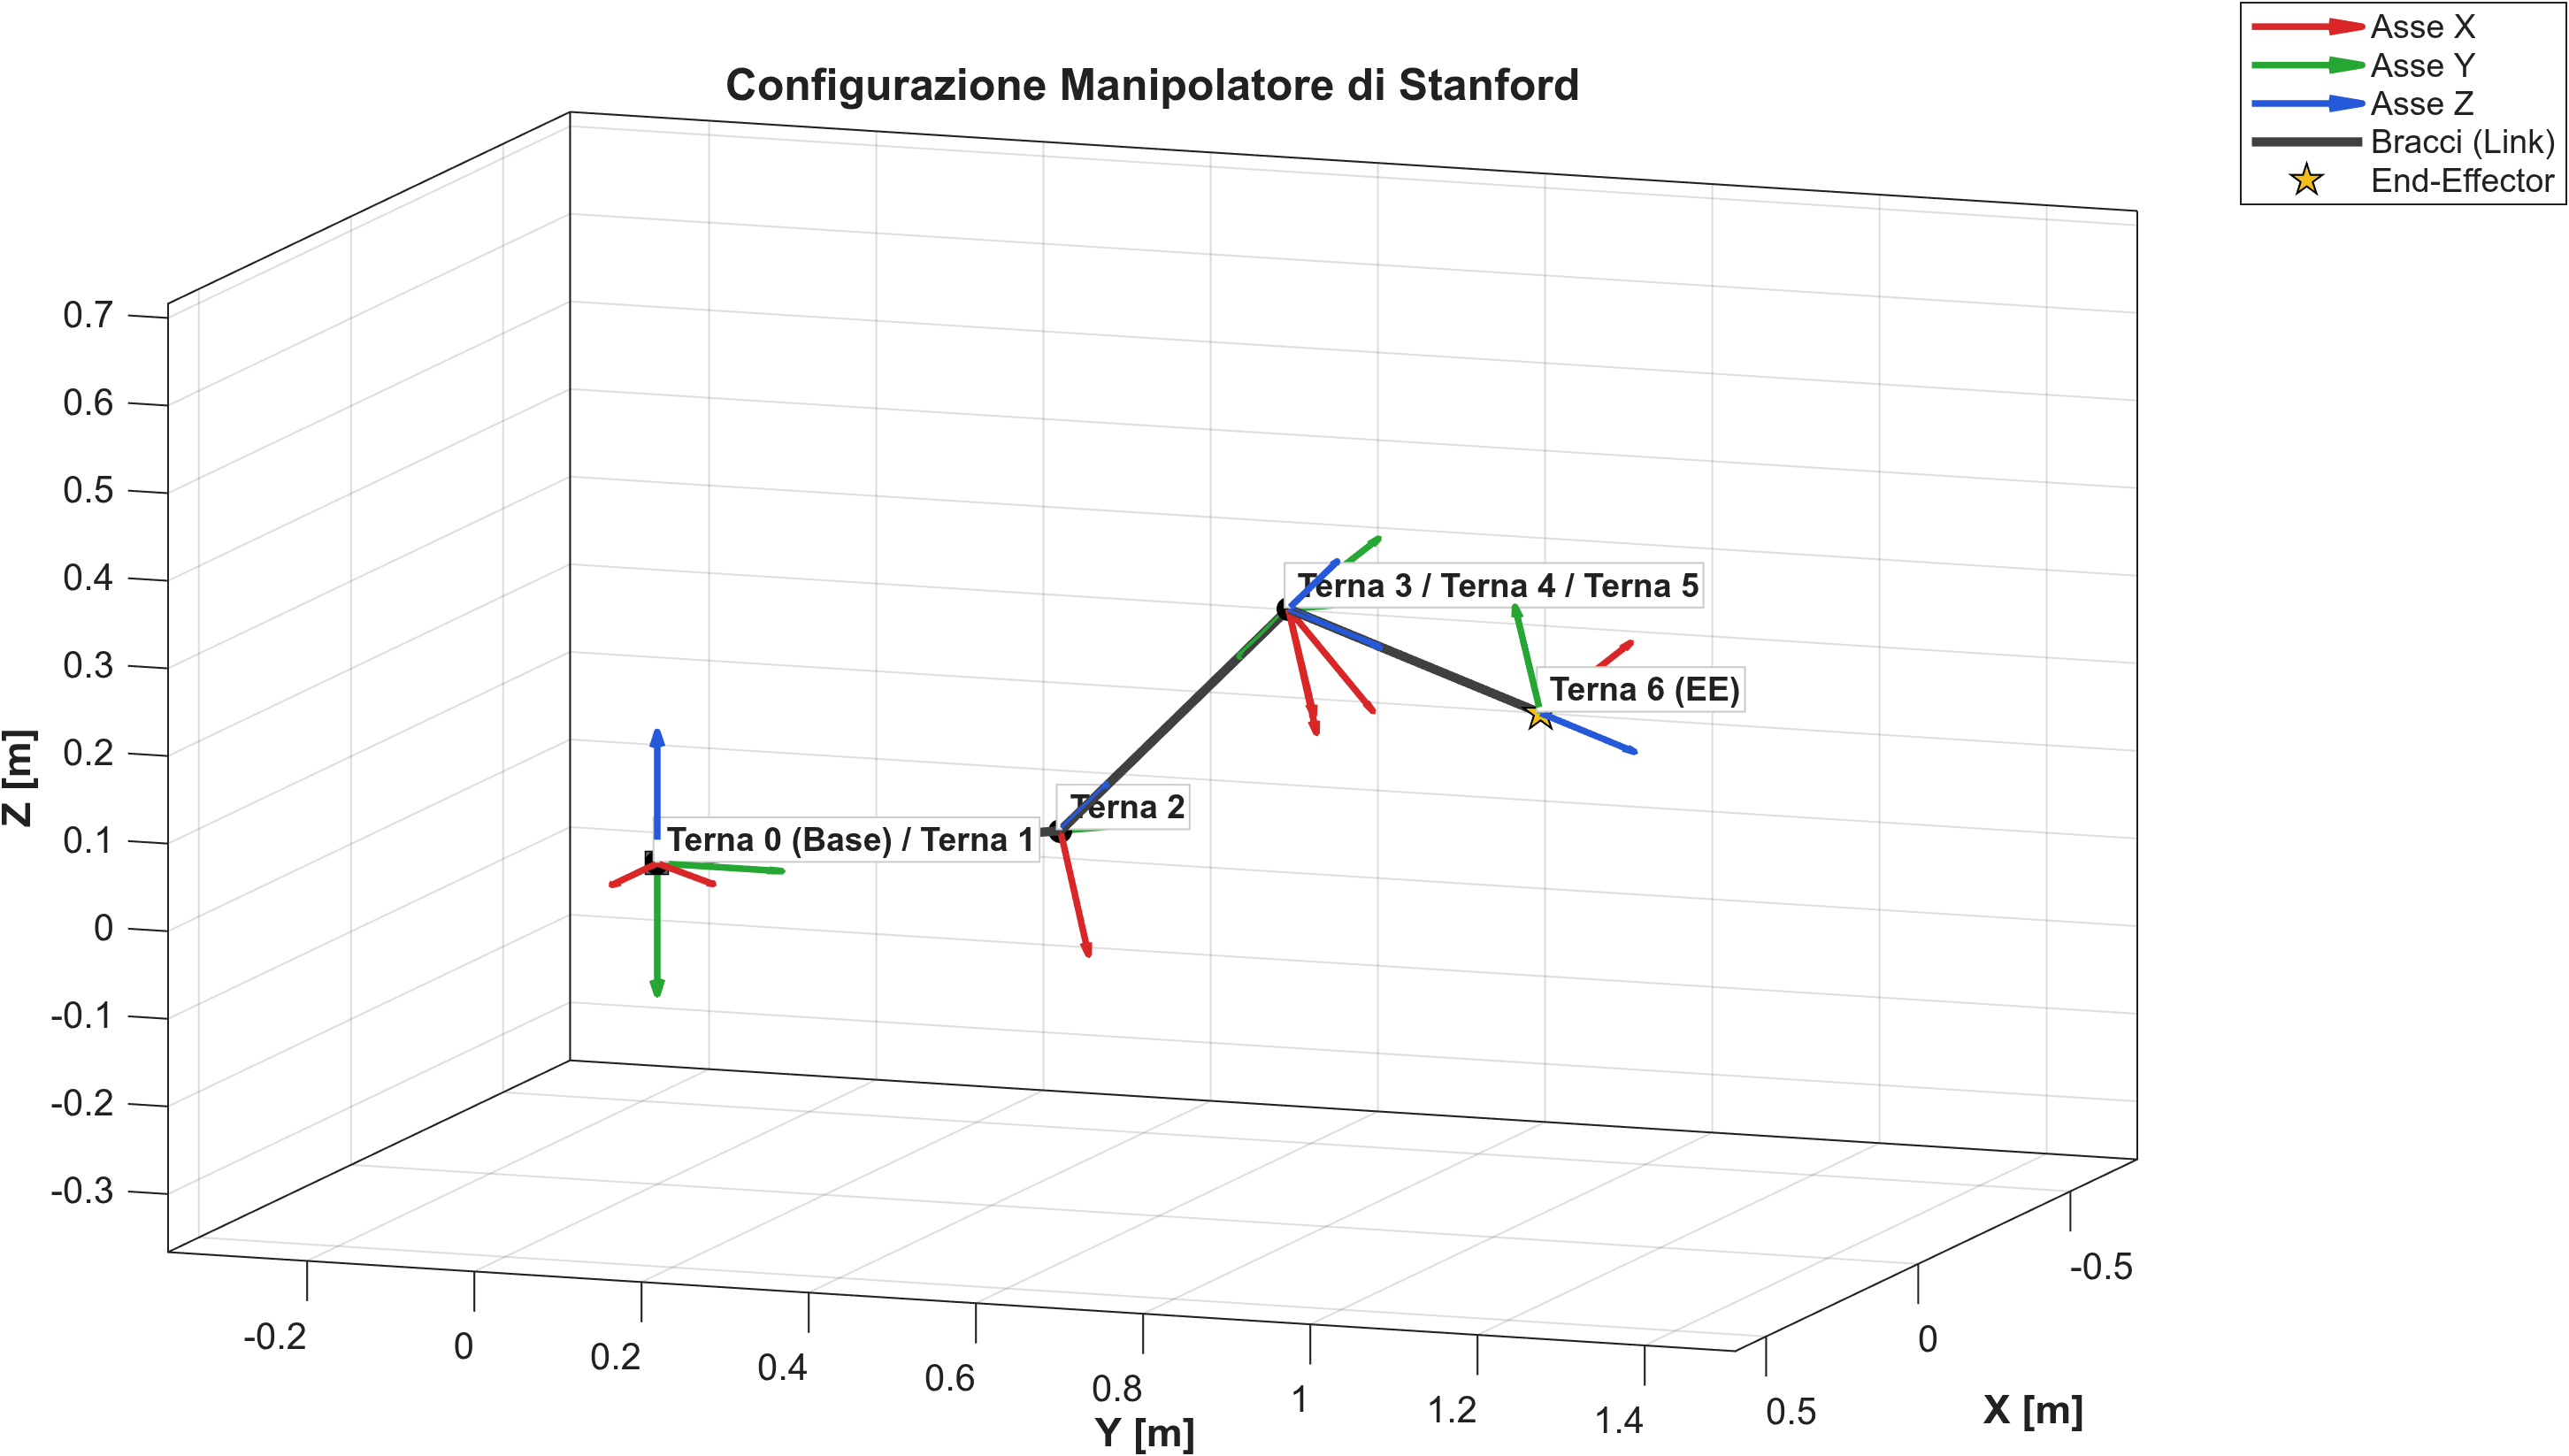
\includegraphics[width=1\linewidth]{E3_6_1_CinematicaDirettaManipolatoreStanford.png}
\end{center}

\end{document}
